\documentclass[18pt,oneside,a4paper, titlepage]{article}

\usepackage[hidelinks]{hyperref}
\usepackage[pdftex]{graphicx}

\begin{document}
\title{\textbf{AOS project}\\ A.Y. 2015/2016\\
	Politecnico di Milano}	
\author{Barlocco Mattia, matr. 873801\\Belotti Nicola, matr. 793419\\Colombo Andrea, matr. 853381}
\date{September, 2016}
\maketitle

\newpage
\tableofcontents

\newpage
\section{Introduction}
	The goal of this project is to recognize which button of a remote control is pushed by using the BPW34 photodiode and the stm32f407. This board has a Analogic to Digital Converter (ADC) built-in that converts the anologic signal received from the BPW to a digital signal. This board operating system is Miosix.
	\begin{figure}[h]
		\centering
		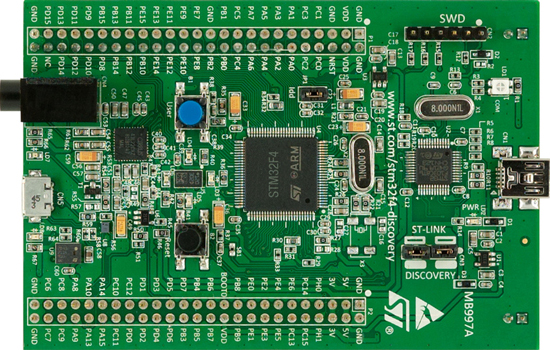
\includegraphics[scale=0.6]{board.jpg}%
	\end{figure}
\newpage
\section{BPW34}
	\begin{figure}[h]
		\centering
		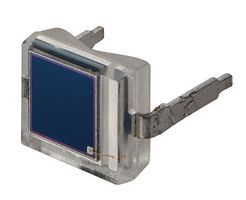
\includegraphics[scale=0.3]{fotodiodo.jpg}
	\end{figure}
	The BPW34 is a photodiode that is sensitive to visible and infrared radiation. Its carateristics are the following:
	\begin{itemize}
		\item It is sensitive at most 34KHz
		\item Fast response times
		\item Angle of half sensitivity: = ± 65°
		\item High photo sensitivity
		\item Suitable for visible and near infrared radiation
	\end{itemize}
	
For any other information on this photodiode visit: \url{http://www.vishay.com/docs/81521/bpw34.pdf}
\newpage
\section{How it works}
	\subsection{Board configuration}
	Used pins are the following:
		\begin{itemize}
			\item GND: BPW34 black wire 
			\item GND: FTDI black wire
			\item PC1: BPW34 red wire 
			\item PB10:FTDI yellow wire 
			\item PB11:FTDI orange wire  
			\item VDD: FTDI red wire 
		\end{itemize}
		The BPW34 sends the value that it sees to the pin PC1. This pin is connected to the ADC, it converts the value in digital so we can use it easly.\\ The FTDI is used to print the values, that the photodiode receives, on the Arduino serial monitor.
	\begin{figure}[h]
		\centering
		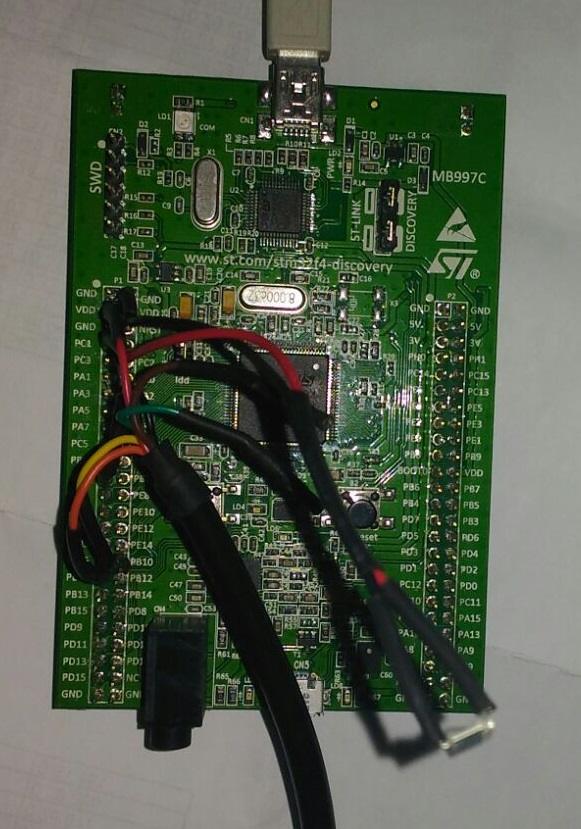
\includegraphics[scale=0.6]{boardLinked.jpeg}
	\end{figure}
	\newpage
	\subsection{Code description}
		We wrote three files of code:
		\begin{itemize}
			\item main.cpp: source file where we wrote the main
			\item adc.h: header file where we define the new class Adc with the constructor the method start() starts a conversion and the method read() waits for the end of the conversion and it returns the digital value
			\item adc.cpp: source file where we wrote the code of the method defined in the adc.h
		\end{itemize}
		In the main.cpp the program starts and we take 200 values of the light of the surrounding space to fix a threshold. After that we monitor the light, and when we receive a value greater then the treshold, we start to save 30000 values in a buffer (the results are illustrated in the next chapter). In this buffer is memorized the code of the button that we pressed. Whenever 
\newpage
		\subsection{Results}

The goal has not been reached. However we have been able to see whether a button is pushed or not.\\
Obviously our project works when a consumer infrared is used, such as remote control for a tv, or a dvd player.\\
We found our system doesn't works on home gate remote controls or car keys because those kind of remote controls use signals out of the infrared trasmission(such as Megaherz transmission).\\
Following images show our sampling on different buttons.

\begin{figure}[h]
	\centering
	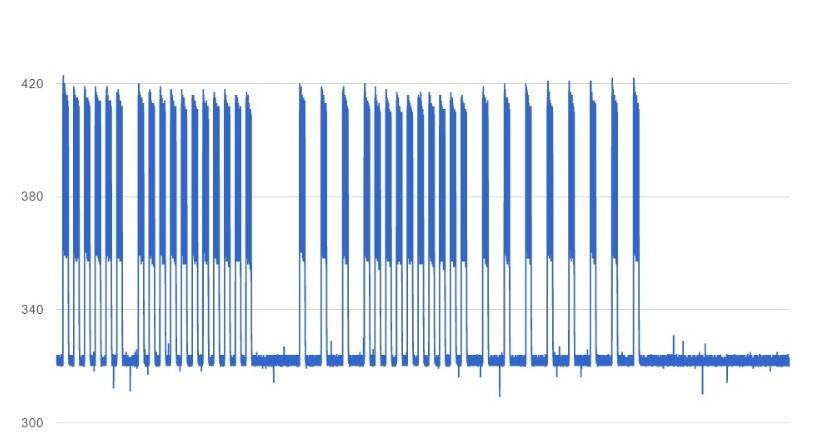
\includegraphics[scale=0.3]{graphs/onButton_2.jpg}%
	\caption{ON button}

\end{figure}

\begin{figure}[h]
	\centering
	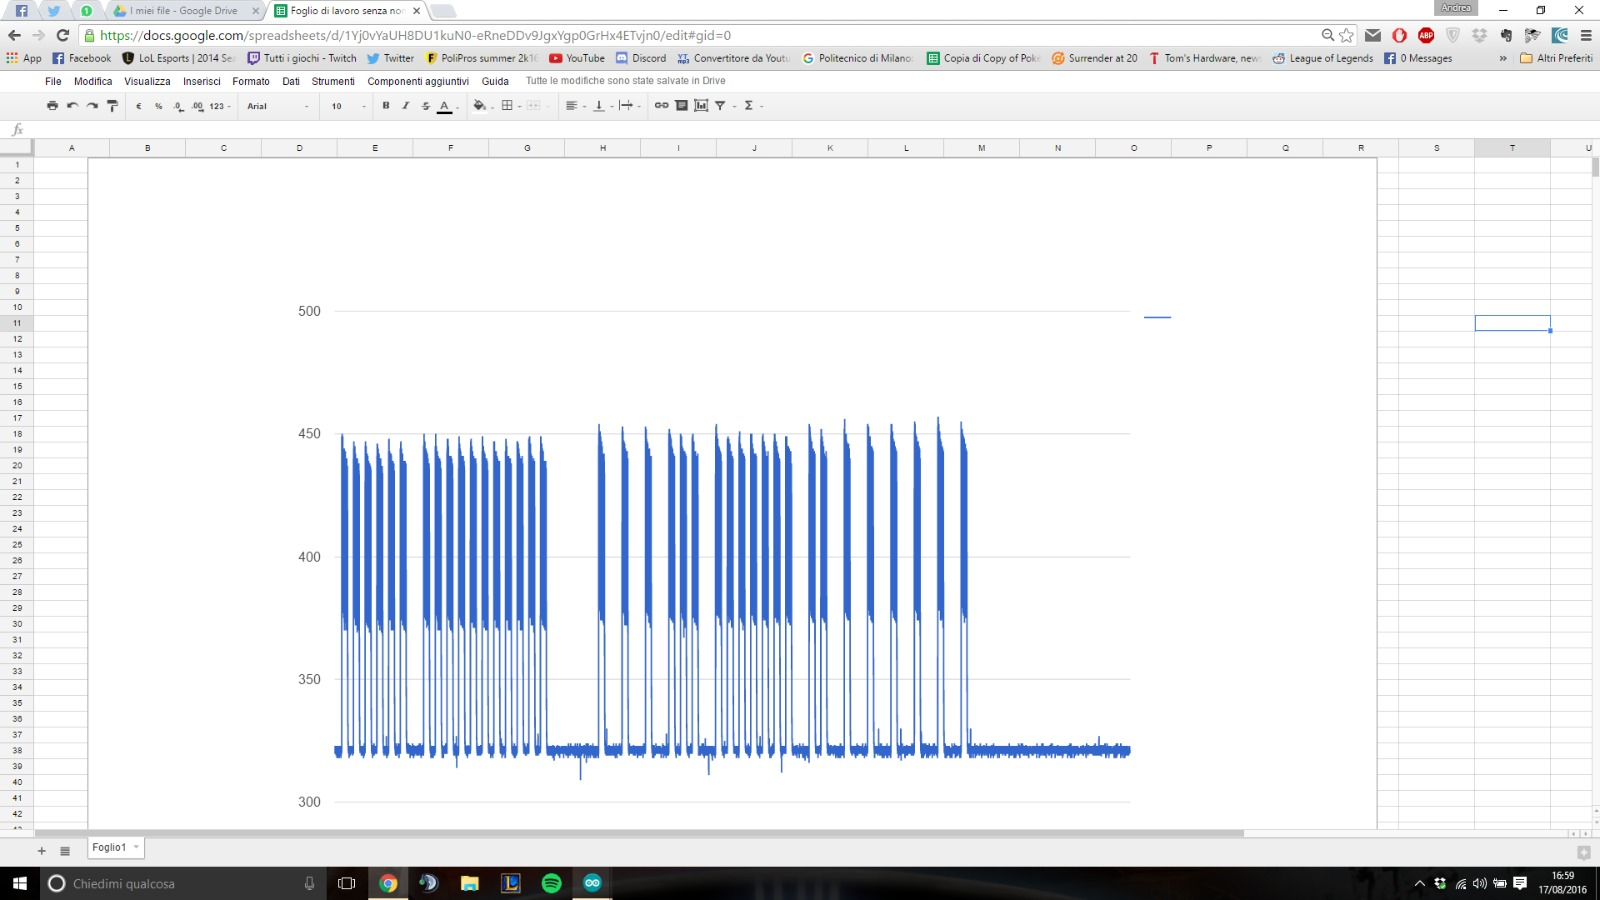
\includegraphics[scale=0.3]{graphs/1Button.jpg}%
	\caption{1 button}
		
\end{figure}

\begin{figure}[h]
	\centering
	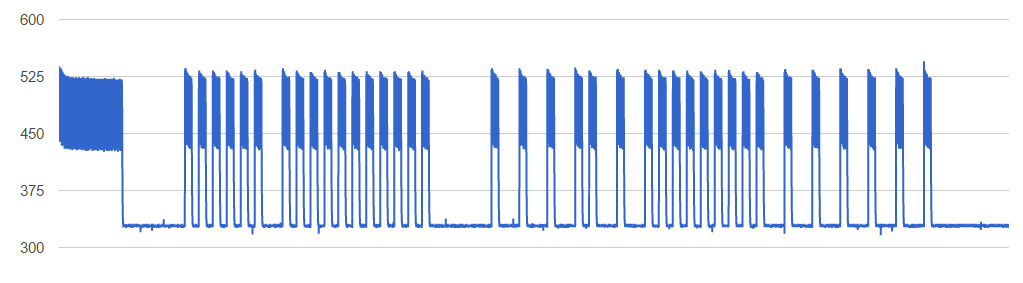
\includegraphics[scale=0.25]{graphs/nonSoIlTasto_1.jpg}%
	\caption{2 button}
	
\end{figure}

\newpage
\section{Used Software}
\begin{itemize}
	\item QSTlink2: used to program the board.
	\item Github: to save every code changes  online.
	\item Latex: to write this document.
	\item Notepad++: to write code.
	\item Miosix Toolchain: to compile the project
	\item ArduinoIDE: serial Arduino monitor 

\end{itemize}

\end{document}